\chapter{Implementasi dan Pengujian}
Bab ini akan berisi tentang implementasi perangkat lunak serta pengujian pada perangkat lunak tersebut. Hasil dari pengujian akan digunakan untuk menarik kesimpulan. 

\section{Implementasi}
Perangkat lunak akan diimplementasikan menjadi sebuah program dengan menggunakan bahasa Java. Rancangan antarmuka yang telah dijelaskan pada Bab \ref{perancangan_antarmuka}, telah berhasil diimplementasikan dan dapat dilihat pada gambar-gambar di bawah ini.

\begin{figure}[H]
	\centering
	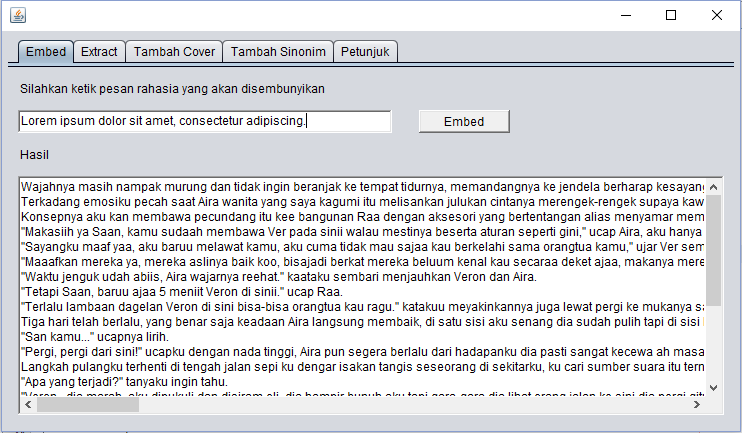
\includegraphics[scale=0.8]{Gambar/ui-embed}
	\caption{Tampilan \textit{tab Embed}} 
	\label{fig:ui-embed}
\end{figure}

\begin{figure}[H]
	\centering
	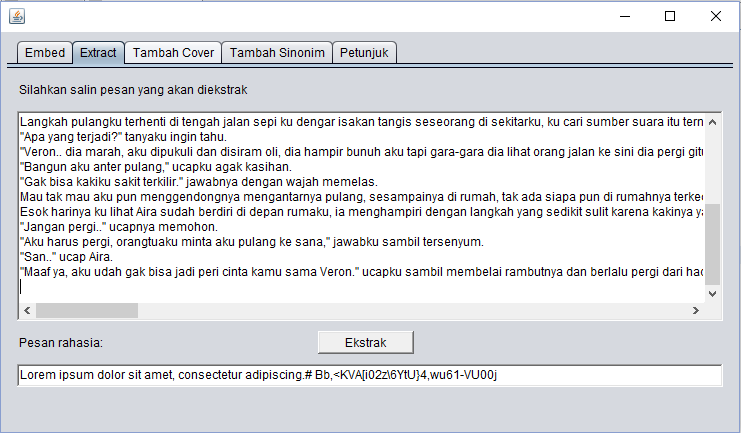
\includegraphics[scale=0.8]{Gambar/ui-extract}
	\caption{Tampilan \textit{tab Extract}} 
	\label{fig:ui-extract}
\end{figure}

Gambar \ref{fig:ui-extract} menunjukkan bahwa ada karakter '\#' yang memberitahu penerima bahwa pesan rahasia telah berakhir, seperti yang telah dijelaskan pada Bab \ref{algoritma}.

\begin{figure}[H]
	\centering
	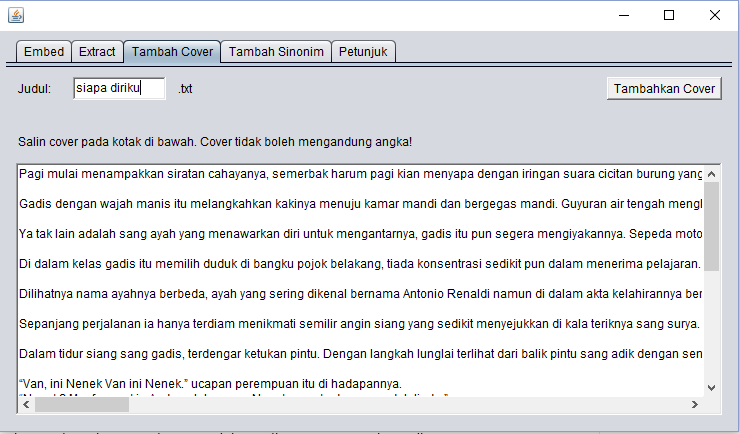
\includegraphics[scale=0.8]{Gambar/ui-tambah-cover}
	\caption{Tampilan \textit{tab Tambah Cover}} 
	\label{fig:ui-tambah-cover}
\end{figure}

\begin{figure}[H]
	\centering
	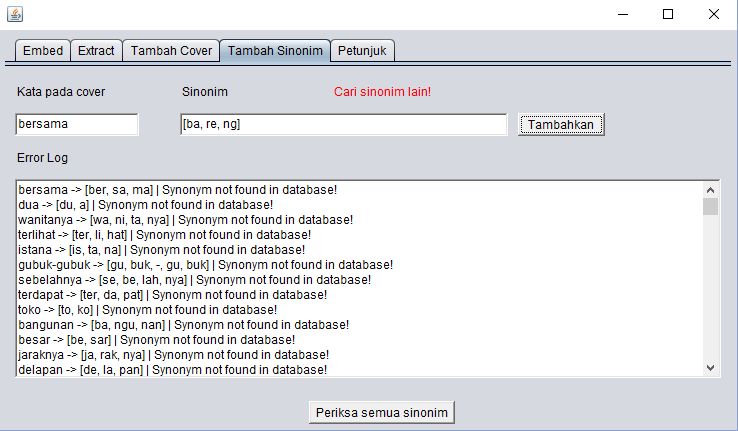
\includegraphics[scale=0.8]{Gambar/ui-tambah-sinonim}
	\caption{Tampilan \textit{tab Tambah Sinonim}} 
	\label{fig:ui-tambah-sinonim}
\end{figure}

Gambar \ref{fig:ui-tambah-sinonim} merupakan contoh saat pengirim memasukkan pasangan kata dan sinonim yang memiliki \textit{c}(\textit{w}) yang memiliki nilai yang sama. Seperti yang telah dijelaskan pada Bab \ref{perancangan_antarmuka}, jika penambahan sinonim gagal, \textit{textbox} sinonim akan diisi dengan hasil pemenggalan kata oleh perangkat lunak. Hal ini dilakukan untuk memberitahu pengirim bagaimana perangkat lunak memenggal kata tersebut. Pemenggalan kata yang dilakukan oleh perangkat lunak tidak sempurna, namun hal ini tidak menjadi masalah karena yang terpenting pemenggalan katanya konsisten.

\begin{figure}[H]
	\centering
	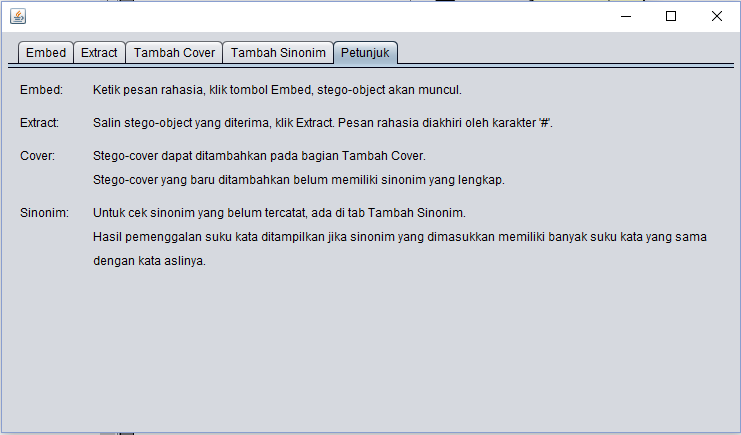
\includegraphics[scale=0.8]{Gambar/ui-petunjuk}
	\caption{Tampilan \textit{tab Petunjuk}} 
	\label{fig:ui-petunjuk}
\end{figure}

\section{Pengujian}
Pengujian yang dilakukan adalah pengujian fungsional dan pengujian eksperimental. Pengujian ini dilakukan untuk memeriksa apakah perangkat lunak yang dibuat telah berfungsi dengan baik. Hasil pengujian ini juga akan dipakai untuk menarik kesimpulan pada bab terakhir.

\subsection{Pengujian Fungsional}
Pengujian fungsional dilakukan untuk memeriksa apakah perangkat lunak memberikan reaksi yang seharusnya terhadap aksi dari pengguna perangkat lunak. Pengujian ini dilakukan pada sistem operasi Windows. Terdapat beberapa tes kasus yang diujikan kepada setiap fungsinya, untuk lengkapnya dapat dilihat pada tabel masing-masing di bawah ini.\\

\begin{table}[H]
\label{table-fungsional-embed}
\centering
\caption{Tabel Pengujian Fungsional \textit{Embed}}
\begin{tabular}{|p{0.3cm} | p{4.5cm} | p{7cm} | p{2.5cm} |}\hline
No. & Aksi & Reaksi seharusnya & Hasil\\
\hline
1 & Pengguna mengetikkan pesan rahasia sepanjang 100 karakter lalu menekan tombol Embed (panjang karakter pesan rahasia masih dapat ditampung \textit{stego-cover} yang ada.) & Perangkat lunak menampilkan \textit{stego-cover} & Sesuai\\
2 & Pengguna mengetikkan pesan rahasia sepanjang 200 karakter lalu menekan tombol Embed (panjang karakter pesan rahasia tidak dapat ditampung \textit{stego-cover} yang ada.) & Perangkat lunak menampilkan \textit{stego-cover} & Perangkat lunak menampilkan teks "Pesan rahasia melebihi kapasitas yang ada!"\\
3 & Pengguna mengetikkan pesan rahasia yang mengandung karakter yang tidak didukung perangkat lunak & Perangkat lunak menampilkan \textit{stego-cover} & Sesuai \\
\hline
\end{tabular}
\end{table}

\begin{table}[H]
\label{table-fungsional-extract}
\centering
\caption{Tabel Pengujian Fungsional \textit{Extract}}
\begin{tabular}{|p{0.3cm} | p{4.5cm} | p{7cm} | p{2.5cm} |}\hline
No. & Aksi & Reaksi seharusnya & Hasil\\
\hline
1 & Pengguna memasukkan \textit{stego-object} lalu menekan tombol Extract & Perangkat lunak menampilkan pesan rahasia, karakter '\#' menandakan pesan rahasia telah berakhir & Sesuai \\
2 & Pengguna memasukkan teks yang bukan \textit{stego-object} lalu menekan tombol Extract & Perangkat lunak menampilkan pesan bahwa tidak ada pesan rahasia dalam \textit{stego-object} yang dimasukkan & Sesuai \\
3 & Pengguna memasukkan \textit{stego-object} yang merupakan hasil \textit{embed} pesan rahasia yang mengandung karakter yang tidak didukung perangkat lunak & Perangkat lunak menampilkan pesan rahasia & Perangkat lunak menampilkan pesan rahasia namun tidak sesuai dengan pesan rahasia yang disembunyikan.\\
\hline
\end{tabular}
\end{table}

Pada Tabel \ref{table-fungsional-extract}, dapat dilihat bahwa pada nomor 3 menampilkan pesan rahasia yang tidak sesuai dengan yang disembunyikan. Hal tersebut terjadi karena saat proses \textit{embed}, karakter yang tidak terdaftar tersebut bisa saja memiliki ASCII yang lebih dari 7 bit, sehingga pada saat ekstraksi, hanya 7 bit pertama dari karakter tersebut yang diekstraksi. Hasilnya pesan yang diekstrak tidak sesuai. 

\begin{table}[H]
\label{table-fungsional-tambah-cover}
\centering
\caption{Tabel Pengujian Fungsional Tambah Cover}
\begin{tabular}{|p{0.3cm} | p{4.5cm} | p{7cm} | p{2.5cm} |}\hline
No. & Aksi & Reaksi seharusnya & Hasil\\
\hline
1 & Pengguna memasukkan \textit{stego-cover} dan judul yang belum terdaftar & Perangkat lunak membuat \textit{file stego-cover} yang baru dan mendaftarkannya pada \textit{stego-cover list} & Sesuai\\
2 & Pengguna memasukkan \textit{stego-cover} tanpa memasukkan judul & Perangkat lunak menampilkan pesan bahwa judul belum diisi & Sesuai \\
3 & Pengguna memasukkan \textit{stego-cover} dengan judul yang sudah terdaftar & Perangkat lunak menampilkan pesan bahwa judul sudah terdaftar & Sesuai \\
4 & Pengguna memasukkan judul yang belum terdaftar, tetapi \textit{stego-cover} yang dimasukkan sudah pernah ditambahkan & Perangkat lunak membuat \textit{file stego-cover} yang baru dan mendaftarkannya pada \textit{stego-cover list} & Sesuai \\
\hline
\end{tabular}
\end{table}

Pada Tabel \ref{table-fungsional-tambah-cover}, dapat dilihat bahwa untuk kasus pada nomor 4, \textit{stego-cover} tetap ditambahkan. Hal ini dikarenakan perangkat lunak hanya memeriksa apakah judul yang dimasukkan pengguna sudah terdaftar atau belum, tanpa memeriksa isi dari \textit{stego-cover} yang dimasukkan pengguna.

\begin{table}[H]
\label{table-fungsional-tambah-sinonim}
\centering
\caption{Tabel Pengujian Fungsional Tambah Sinonim}
\begin{tabular}{|p{0.3cm} | p{4.5cm} | p{7cm} | p{2.5cm} |}\hline
No. & Aksi & Reaksi seharusnya & Hasil \\
\hline
1 & Pengguna menambahkan kata dan sinonim dengan nilai \textit{c}(\textit{w}) yang berbeda & Perangkat lunak menambahkan sinonim ke kamus sinonim & Sesuai \\
2 & Pengguna menambahkan kata dan sinonim dengan nilai \textit{c}(\textit{w}) yang sama & Perangkat lunak menampilkan peringatan dan hasil pemenggalan sinonim & Sesuai \\
\hline
\end{tabular}
\end{table}

\begin{table}[H]
\label{table-fungsional-cek-sinonim}
\centering
\caption{Tabel Pengujian Fungsional Cek Semua Sinonim}
\begin{tabular}{|p{0.3cm} | p{4.5cm} | p{7cm} | p{2.5cm} |}\hline
No. & Aksi & Reaksi seharusnya & Hasil \\
\hline
1 & Pengguna memeriksa semua sinonim (ada kata yang sinonimnya belum terdaftar) & Perangkat lunak menampilkan kata-kata yang sinonimnya tidak terdaftar pada kamus sinonim & Sesuai\\
2 & Pengguna memeriksa semua sinonim (semua kata sudah terdaftar sinonimnya) & Perangkat lunak tidak menampilkan apa pun & Sesuai \\
\hline
\end{tabular}
\end{table}

\subsection{Pengujian Eksperimental}
Pengujian eksperimental ini dilakukan untuk meneliti waktu dari respon perangkat lunak terhadap beberapa kasus. Dapat dilihat pada Gambar \ref{fig:graf-embed} grafik perbandingan antara waktu yang dibutuhkan untuk \textit{embed} pesan rahasia yang pendek sampai yang panjang.

\begin{figure}[H]
	\centering
	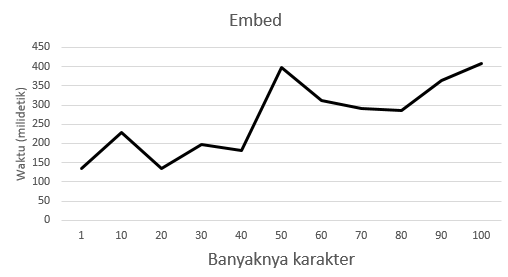
\includegraphics[scale=0.8]{Gambar/graf-embed}
	\caption{Grafik waktu yang dibutuhkan \textit{embed} pesan rahasia} 
	\label{fig:graf-embed}
\end{figure}

\begin{figure}[H]
	\centering
	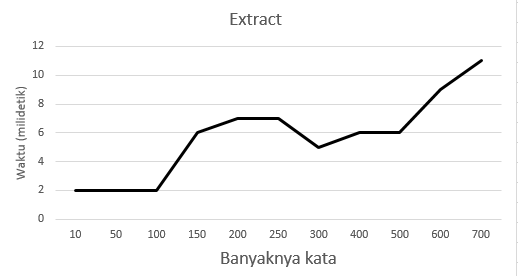
\includegraphics[scale=0.8]{Gambar/graf-extract}
	\caption{Grafik waktu yang dibutuhkan \textit{extract stego-object}} 
	\label{fig:graf-extract}
\end{figure}

Dapat dilihat pada Gambar \ref{fig:graf-extract} grafik perbandingan antara waktu yang dibutuhkan untuk \textit{extract}. Waktu yang dibutuhkan untuk melakukan ekstraksi memang berbanding lurus dengan banyak kata pada \textit{stego-object}, namun perbedaannya pun tidak terlalu jauh.

\begin{figure}[H]
	\centering
	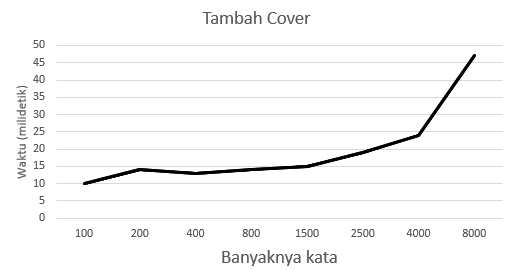
\includegraphics[scale=0.8]{Gambar/graf-tambah-cover}
	\caption{Grafik waktu yang dibutuhkan untuk menambahkan \textit{cover}} 
	\label{fig:graf-tambah-cover}
\end{figure}

Gambar \ref{fig:graf-tambah-cover} menunjukkan bahwa waktu yang dibutuhkan untuk menambahkan \textit{cover} tidaklah lama, karena perangkat hanya membuat \textit{file} baru dan menulis apa yang dimasukkan pengguna. Jika dilihat dari tiga grafik di atas, waktu yang paling lama adalah proses \textit{embed}, dikarenakan selain memenggal kata, proses \textit{embed} juga harus membaca \textit{file} kamus sinonim untuk memodifikasi \textit{stego-cover}.